\section{Алгоритм извлечения антропометрических признаков из видео}

Процесс извлечения антропометрических признаков включает следующие этапы:

\begin{itemize}
	\item Предварительная обработка и нормализация изображения: на этом этапе необходимо выполнить фильтрацию шума и сглаживание изображения, применить морфологические операторы для улучшения качества контура объекта, для увеличения диапазона яркости изображений провести эквализацию их гистограмм (представлено в разделе \ref{part2.2.1});
	\item Использование алгоритма вычитания фона для обнаружения объектов: На этом шаге применяется два различных алгоритма: вычитание фона и на основе метода порогового значения. Применение для изображений и видео, полученных с камеры (представлено в разделе в \ref{part2.2.2});
	\item Использование алгоритма сегментации изображений и поиска ближайших точек границы чтобы найти местонахождение и контуры частей человеческого тела. На этом шаге применяется алгоритм разреза на графах для сегментации изображений и поиска частей человеческого тела, алгоритм обнаружения контура, итеративный алгоритм ближайших точек (Iterative Closest Point-$ICP$) для определения и корректировки точек признаков, которые ближе всего к их фактическим границам;
	\item Сравнительный анализ извлеченых признаков с реальными объектами для проверки точности методов и алгоритмов компьютерного зрения: на этом этапе будут сравниваться геометрические особенности частей человеческого тела с их настоящими частями, размеры которых были извлечены из реального тела, чтобы настроить соответствующие параметры.
\end{itemize}

В данной работе предложен метод извлечения антропометрических признаков из изображений и видео на основе алгоритмов компьютерного зрения предложенного подхода к задаче автоматического извлечения антропометрических признаков в режиме реального времени.


\subsection{Предварительная обработка изображения} \label{part2.2.1}
\subsubsection{Фильтрация изображений с помощью гауссового фильтра}
Шум является неотъемлемой частью любого устройства регистрации изображений и видео. Условно можно выделить следующие виды шума:

\begin{itemize}
	\item Шум  устройств захвата изображения;
	\item Смаз изображения, связанный с условиями регистрации, включая скорость и траекторию движения камеры;
	\item Независимый случайный шум;
	\item Отдельно отметим вмешательство наблюдения объектов.
\end{itemize}

В основе математической теории обработки изображений, включая фильтрацию, лежит понятие свертки (convolution) c определенным ядром (kernel, маска фильтра). Для того, чтобы выполнить преобразование была проведена «свертка» входного изображения с соответствующим (заранее выбранным) ядром. Со всеми пикселями в изображении проводятся свертка с ядром свертки (\ref{eq1}) (центр окна свертки будет размещен в позиции пикселя, вычисляется свертка), изменение исходных значений пикселей.
\begin{equation}\label{eq1}
Y\left(m,n\right)=X\left(m,n\right)\ast H\left(k,l\right)=\sum^r_{k=-r}\sum^r_{l=-r}X\left(m-k,n-l\right)H\left(k,l\right),
\end{equation}

\begin{itemize}
	\item $X\left(m,n\right)$ - исходная матрица размера изображения $m\ast n$;
	\item $H\left(k,l\right)$ - матрица ядра свертки, также известная как маска;
	\item $Y\left(m,n\right)$ - выходная матрица свертки между $X$ и $H$.
\end{itemize}

В данной работе использован фильтр Гаусса для удаления шума. Сущность этого преобразования состоит в реализации свертки оригинального изображения с ядром симметричной формы в виде 2-D функции Гаусса. Эта непрерывная функция определяется следующим образом:
\begin{equation}\label{eq2}
f\left(x,y\right)=\frac{1}{2\pi\sigma^2}exp\left(-\frac{x^2+y^2}{2\sigma^2}\right).
\end{equation}

Теория линейной и нелинейной фильтрации изображений является областью проведения активных научных исследований \cite{Sizikov2011,Sizikov260,Sizikov2012}.
\subsubsection{Метод бинарной морфологии}
В настоящее время методы цифровой обработки изображений привлекли внимание многих исследователей и разработчиков. Отдельно отметим метод морфологической обработки изображений.

Морфологическая обработка изображений дает количественное описание структуры и геометрии объектов в изображении, основанной на математической теории, таких как теории множеств, топологии, теории вероятности и т.д.

В приложениях компьютерного зрения морфологическая обработка используется для идентификации объектов, повышении качества изображения, сегментации изображения и проверки ошибок на изображении. Операции морфологической обработки выполняются в основном на бинарном изображении.

\textbf{Структурные элементы} \cite{Burger2009}.  В бинарном изображении, Структурный элемент представляет собой небольшое изображение, состоящий из двух значений $0$ и $1$, при этом $0$ значения игнорируются в процессе вычисления, $H\left(i,j\right)$ является структурные элементы бинарного изображения и выражается следующим образом: $H\left(i,j\right) \in \left\{0,1\right\}$.

Некоторые формы структурных элементов, обычно используемые в бинарном изображении: горизонтальные и вертикальные линии, квадраты, эллипсы и пр.

\begin{figure}[ht!]
\centering
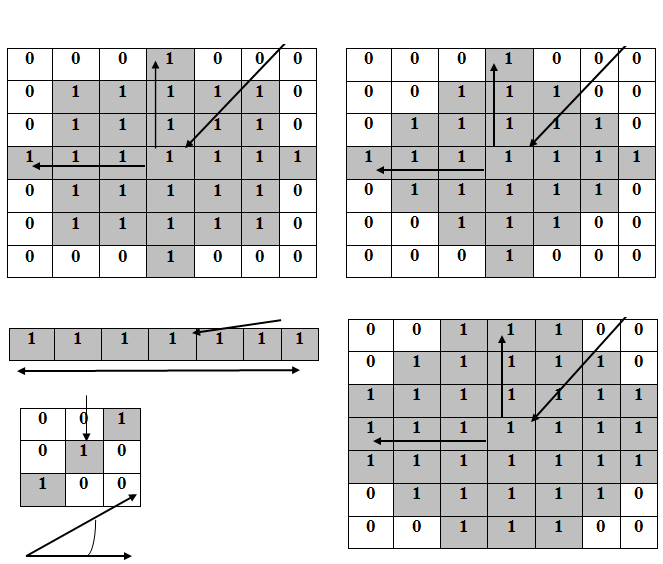
\includegraphics [scale=0.8] {images/h8.png}
\begin{center}
%\captionsetup{justification=justified, labelsep=period}
\caption{Описание формы структурных элементов.} \label{img8}
\end{center}
\end{figure}
Цель метода морфологической обработки - найти связанные компоненты контура объекта для получения идеального контура.

Операции дилатации, эрозии, открытия и закрытия могут быть применены для серого изображения. Эта концепция аналогична для бинарных морфологических операций.
\begin{equation}\label{eq3}
 g=\left(f\oplus b \right)-\left(f\ominus b\right),
\end{equation}
Где:

\begin{itemize}
	\item $f\oplus b$ является преобразованием расширения растяжением $f$ по структурным элементам b в положении $\left(x,y\right)$ по формуле:
	\begin{equation}\label{eq4}
\left[f\oplus b\right]\left(x,y\right)=max_{\left(s,t\right)\in b}\left\{f\left(x-t,y-t\right)\right\}.
\end{equation}
\item $f \ominus b$ является преобразованием эрозии растяжением $f$ по структурным элементам b в положении $\left(x,y\right)$ по формуле:
	\begin{equation}\label{eq5}
\left[f \ominus b\right]\left(x,y\right)=max_{\left(s,t\right)\in b}\left\{f\left(x+t,y+t\right)\right\}.
\end{equation}
\end{itemize}
Набор пикселей, которые соединяются с другими называется компонентой связности \cite{Solomon2011}. Пиксели соединены друг с другом, которые отличаются от других групп пикселей назначенной им меткой. Эти метки представляют собой целые числа, где фон имеет значение $0$, область изображения $/$ группа взаимосвязанных пикселя помечена $1$.
\begin{figure}[ht!]
\centering
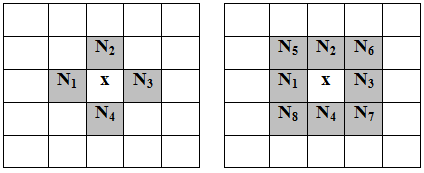
\includegraphics [scale=0.8] {images/h9.png}
\begin{center}
%\captionsetup{justification=justified, labelsep=period}
\caption{Форма 4 соседей (N4) и 8 соседей (N8).} \label{img9}
\end{center}
\end{figure}
В данной работе используются алгоритмы для обозначения 8-связных компонент (рис.\ref{img9}). Алгоритм включает в себя следующие этапы:

\begin{itemize}
	\item Шаг 1: Сканирование входных изображений последовательно по строкам сверху-внизу, чтобы встретить любую точку $p$ $\left(p=1,если бинарное изображен\right)$ в изображении;
	\item Шаг 2: Проверка соседей $p$. На основе этой информации, метка будет осуществляться следующим образом:
	
	\begin{itemize}
		\item Если все соседи со значением равным нулю, то $p$ присваивается новая, ранее не использовавшаяся метка.
		\item Если имеется только один соседний пиксел $р$ со значением $1$, присваиваем эту метку пикселу $р$;
		\item Если имеется больше чем один соседний пиксел $р$ со значением $1$, присваиваем метку любого из уже пронумерованных пикселов.
	\end{itemize}
	
\end{itemize}
После завершения процесса сканирования, соответствующие пары метки располагаются в соответствующие группы, и каждой группе будет присвоена только одна метка.
\subsubsection{Метод выравнивания гистограммы}
При регистрации изображений и видео при помощи всегда происходит дисбаланса света. Эта проблема может быть легко решена путем воздействия на источник света в случае лабораторных условиях регистрации.

Настоящая работа направлена на создание практических приложений для смартфонов, которые могут работать в реальных условиях освещения. Таким образом, автоматический баланс яркости является необходимым требованием для разрабатываемого комплекса программ. Используется метод эквализации гистограммы для решения задачи.

Эквализация гистограммы является простой теорией и часто используется при обработке изображений. Цель эквализации гистограммы, как уже отмечалось выше, заключается в увеличении диапазона яркости изображения.

Эквализация гистограммы изображения g определяется следующим образом:
\begin{equation}\label{eq6}
g_{i,j}=floor\left(\left(L-1\right)\sum^{f_{i,j}}_{n=0}p_n\right),
\end{equation}
Где:

\begin{itemize}
	\item $f$ - исходное изображение;
	\item $n=0,1,…,L-1;L \in \left[0 ; 255\right]$;
	\item $p_n$:Количество пикселей по интенсивности  n / Количество пикселей;
	\item $floor()$ округляется до ближайшего целого числа. Это эквивалентно преобразованию интенсивности пикселей, $k$, $f$ с помощью функции:
	\begin{equation}\label{eq7}
T\left(K\right)=floor\left(\left(L-1\right)\sum^k_{n=0}p_n\right).
\end{equation}
\end{itemize}
Этот метод имеет преимущество простоты, легкости применения, без каких-либо серьезных расчетов, он используется в случаях, когда необходимо привести изображение в его <<нормальное>> состояние.

%-------------------------
\subsection{Алгоритмы вычитания фона изображения для обнаружения объектов в видео} \label{part2.2.2}
Вычитание фона является одним из наиболее популярных используемых алгоритмов в области компьютерного зрения. Алгоритм используется для определения пикселей движущихся объектов в видео, также известных как передний план (FG - foreground), в то время как неподвижный объект называется фоном (BG - background). Алгоритм вычитания фона используется на этапе предварительной обработки в многих задачах компьютерного зрения, результаты этого шага могут существенно повлиять на исход следующих шагов (идентификация, отслеживание, и т.д.).

В данной работе представлены решения для задачи вычитания фона, такие как построение модели на основе гауссовой смешанной модели.

Эта модель используется чтобы обнаружить движущиеся объекты в текущем кадре. Проведено много исследований по методу построения моделирования фона, например в \cite{Mittal2004} авторы использовали адаптивную плотность оценки (adaptive kernel density estimation) и получили хорошие результаты, однако, существует недостатки: требуется большой объем дискового пространства, вычислительная сложность, скорость работы не соответствует реальному времени. В работе \cite{Stauffer2009} Стауффер использовал гауссову смесь (Mixture of Gaussian) в построении модели фона для обнаружения движения. 

Основная идея алгоритма вычитания фона следующая. Пиксель в положении $x$ в изображении принадлежит объекту, если она удовлетворяет неравенству:

	\begin{equation}\label{eq8}
\left|I_n\left(x\right)-B_n\left(x\right)\right| \geq T_n\left(x\right),
\end{equation}

Где:

\begin{itemize}
	\item $I_n\left(x\right) \in \left[0,255\right]$  - значение интенсивности серого в позиции пикселя $x$ принадлежит $n$-му изображению или видеофрагменту;
	\item $B_n \left(x\right)$  - значение интенсивности фона в местоположении пикселя $x$;
	\item $T_n \left(x\right)$  - пороговое значение задается для каждого изображения. 
\end{itemize}
Модель базового фона постоянно обновляется из исходных изображений или видео. На месте расположения пикселей на изображении, разные кадры будут давать разные значения. Например, значение пикселя в позиции х на изображении фона отличается от значения пикселя в позиции х на изображении переднего плана.
\begin{equation}\label{eq9}
B_{n+1}\left(x\right)= \left\{\begin{array}{l} \alpha B_n\left(x\right)+\left(1-\alpha\right)I_n\left(x\right),x\in BG,\\
\beta B_n\left(x\right)+\left(1-\beta\right)I_n\left(x\right),x\in FG,
\end{array}\right.
\end{equation}
где BG - соответствует фону, а FG - переднему плану. Пороговое значение пикселя в позиции $x$ является:
\begin{equation}\label{eq10}
T_{n+1}\left(x\right)= \left\{\begin{array}{l} \alpha T_n \left(x\right)+\left(1-\alpha\right) \left(\left|I_n\left(x\right)-B_n\left(x\right)\right|\right), x \in BG,\\
T_n\left(x\right), x\in FG,
\end{array}\right.
\end{equation}

Параметры $\alpha$, $\beta$ выбираются из интервала $\left[0,1\right]$ для обеспечения обновления фона в изображении и видео. Блок схема алгоритма вычитания фона на основе пороговых значений представлена на (рис. \ref{img10}), а алгоритм обновления фона - на (рис. \ref{img11}).

\begin{figure}[ht!]
\centering
\begin{center}
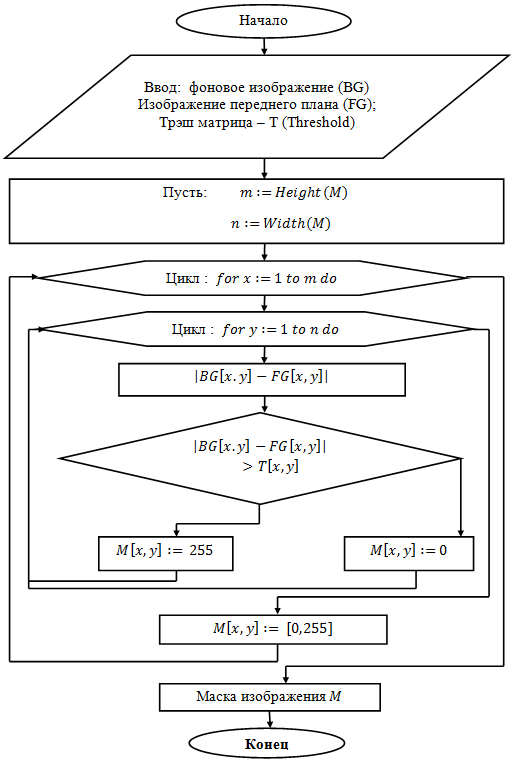
\includegraphics [scale=1] {images/h10.png}
%\captionsetup{justification=justified, labelsep=period}
\caption{Блок-схема алгоритма вычитания фона.} \label{img10}
\end{center}
\end{figure}

\begin{figure}[ht!]
\centering
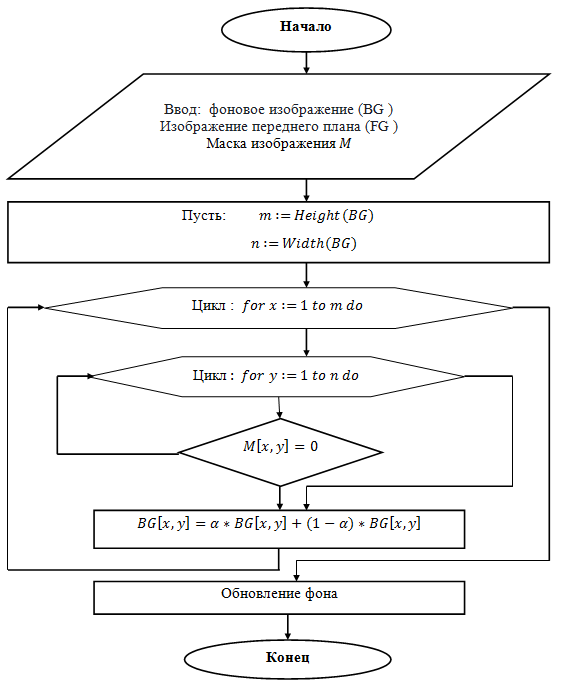
\includegraphics [scale=1] {images/h11.png}
\begin{center}
%\captionsetup{justification=justified, labelsep=period}
\caption{Блок-схема алгоритма обновления фона.} \label{img11}
\end{center}
\end{figure}

Каждый пиксель моделируется как случайный вектор. Значение пикселя $x$ в момент времени $t : x^{\left(t\right)}$. Значения пикселей на основе распределения гауссово смеси:

\begin{equation}\label{eq11}
P\left(0|\theta\right)=\sum^K_{k=1}\pi_kN\left(x|\mu_k,\beta_k\right).
\end{equation}

Для обновления фона в видео, модель фона должна постоянно обновляться, с помощью случайной выборки $X=\left\{x^{\left(t\right)},..., x^{\left(t-T\right)}\right\}$для оценки параметров модели. Метод максимального распределения (Maximize Posteriori) используется для оценки подходящих параметров в гауссовой модели по формуле:
\begin{equation}\label{eq12}
\hat{\theta} = argmax_\theta \left\{\ln p\left(X|\theta\left(K\right)\right)+\ln p\left(\theta\left(K\right)\right)\right\},
\end{equation}
Где:

\begin{itemize}
	\item $K$ параметр модели;
	\item $P\left(\theta\left(K\right)\right)$Функция распределения параметра $\pi\left(K\right)\equiv\left\{\pi_1, ..., \pi_K\right\}$.
\end{itemize}

Согласно \cite{Bishop2006}
\begin{equation}\label{eq13}
\frac{\partial}{\partial\theta}\left\{\ln P\left(X|\theta\left(K\right)\right)+\ln P\left(\theta\left(K\right)\right)+\gamma\left(\sum^K_{k=1}\pi_k-1\right)\right\},
\end{equation}
\begin{equation}\label{eq14}
\longleftrightarrow \frac{\partial}{\partial\theta}\left\{\sum^t_{n=1}ln\left\{\sum^N_{k=1}\pi_kN\left(x^{\left(n\right)}|\mu_k,\beta_k\right)\right\}-\frac{c}{2}\sum^N_{k=1}ln \pi_k + \gamma\left(\sum^K_{k=1}\pi_k-1\right\}\right) = 0,
\end{equation}
Где:
 $c=\frac{N}{2}$, $N$ - каличество параметров для каждой модели компонента \cite{Figueiredo2002}.
\begin{equation}\label{eq15}
\hat{\pi}^{\left(t\right)}_k = \frac{\hat{\pi}^{\left(t\right)}_k\frac{c}{t}}{1-K\frac{c}{t}},
\end{equation}
\begin{equation}\label{eq16}
\mu^{\left(t\right)}_k = \frac{1}{N_k}\sum^t_{n=1}\gamma^{\left(t\right)}\left(z^{\left(n\right)}_k\right)x^{\left(n\right)},
\end{equation}
\begin{equation}\label{eq17}
\beta^{\left(t\right)}_k =\frac{1}{N_k}\sum^t_{n=1}\gamma^{\left(t\right)}\left(z^{\left(n\right)}_k\right)\left(x^{\left(n\right)}-\mu^{\left(n\right)}_k\right)\left(x^{\left(n\right)}-\mu^{\left(n\right)}_k\right)^T.
\end{equation}
Для построения алгоритма обновления фона, необходимо использовать наблюдаемое значение и поэтому предыдущий результат построения обновляется. Уравнение обновления модели описывается следующим образом:
\begin{equation}\label{eq18}
\hat{\pi}^{\left(t+1\right)}_k=\hat{\pi}^{\left(t\right)}_k + \left(t-1\right)^{-1} \left(\frac{\gamma z^{\left(t\right)}_k}{1-K\frac{c}{T}} - \hat{\pi}^{\left(t\right)}_k\right) - \left(1-t\right)^{-1} \frac{\frac{c}{T}}{1-K\frac{c}{T}},
\end{equation}
\begin{equation}\label{eq19}
\hat{\mu}^{\left(t+1\right)}_k = \hat{\mu}^{\left(t\right)}_k + \left(t+1\right)^{-1} \frac{\gamma^{\left(t\right)}z^{\left(t+1\right)}_k}{\hat{\pi}^{\left(t\right)}_k}\left(x^{\left(t+1\right)}-\hat{\mu}^{\left(t\right)}_k\right),
\end{equation}
\begin{equation}\label{eq20}
\hat{\beta}^{\left(t+1\right)}_k = \hat{\beta}^{\left(t\right)}_k + \left(t+1\right)^{-1} \frac{\gamma^{\left(t\right)}z^{\left(t+1\right)}_k}{\hat{\pi}^{\left(t\right)}_k} \left(x^{\left(t+1\right)}-\hat{\mu}^{\left(t\right)}_k\right)\left(x^{\left(t+1\right)}-\hat{\mu}^{\left(t\right)}_k\right)^T - \hat{\beta}^{\left(t\right)}_k.
\end{equation}

Уравнение (\ref{eq18}) строится из (\ref{eq15}) с $\frac{c}{t}=\frac{c}{T}$  с применением гауссовой модели, чтобы обновить модели фона, помочь алгоритму вычитания фона работать быстрее в режиме реального времени и хорошей точности.



%-------------------------
\subsection{Сегментация изображений при помощи разрезов на графах}
Сегментация изображений является одним из важных шагов в процессе компьютерного зрения. Сегментация изображений играет большую роль в анализе изображений и в получении важной информации из изображений.

На практике сегментация изображений имеет две сложные проблемы: слабые границы и структуры. Первая проблема состоит в нахождении слабых границ, когда они являются частью соответствующей границы. Вторая проблемма заключается в разделении сложных структур в изображении \cite{Sagiv2006, Raviv2007}. На самом деле, такие ситуации часто возникают в практике. В этом случае сегментация становится неясной без добавления априорной информации пользователей. Поэтому, использование методов сегментации изображений с учителем широко используется.

В настоящее время существует много алгоритмов предлагаемых для решения задач сегментации изображений. Существует три типа алгоритмов сегментации обучения с учителем, основанных на исходной информации от пользователей:

\begin{itemize}
	\item Первый тип является результатом сегментации на основании желательных границ, например Intelligent Scissors \cite{Mortensen1995};
	\item Второй тип является  результатом сегментации на основании исходных границ, которые находятся близко с желательными границами, например Active Contour \cite{Lankton} и Set Level \cite{Lie2006};
	\item Третий тип является результатом сегментации на основании маркировки пикселей, которые задаются пользователами.
\end{itemize}
Одним из популярных подходов является метод разреза на графах, которые основаны на функции энергии. В этом методе изображение представляется как взвешенный неориентированный граф. Обычно пиксель или группа пикселей ассоциируется вершиной, а веса рёбер определяют (не)похожесть соседних пикселей. Затем граф (изображение) разрезается согласно критерию, созданному для получения «хороших» кластеров. Каждая часть вершин (пикселей), получаемая этими алгоритмами, считается объектом на изображении.

\textbf{Проблема о максимальном потоке} (maximum flow problem): найти поток $f$ такой, что величина потока максимальна. 
\[
f: \sum_u f\left(u\rightarrow v\right)=\sum_wf\left(v\rightarrow w\right). 
\]

Величина потока (value of flow) — сумма потоков из источника.
\[
\left|f\right|:= \sum_w f \left(s\rightarrow w\right) - \sum_u f\left(u\rightarrow s\right).
\]

\textbf{Минимальный разрез} — разрез с минимальной пропускной способностью. 
$C_{min} \left(A,B\right)=\sum_{u\in S, v \in T} W_{uv}$.

Разрез (s-t cut) — разбиение множества всех вершин V на два подмножества $A$ и $B$ таких, что $s\in A $, $t\in B$, причем пересечение $A$ и $B$ равно пустому множеству. Если рассматривать весовые коэффициенты, связанные с каждым узлом в качестве емкости потока, можно показать, что максимальное количество энергии потока от источника равно емкости минимального разреза. Поэтому проблема минимального разреза также известна как проблема максимального потока. Нужно выбрать необходимый поток и необходимый разрез $\left(S, T\right)$, а затем следить неравенством \cite{Boykov12001}:
\begin{equation}\label{eq21}
\left|f\right| = \sum_w f\left(s\rightarrow w\right) - \sum_u f \left(u\rightarrow s\right),
\end{equation}
\[
=\sum_{v\in S}\left(\sum_w f \left(v \rightarrow w \right) - \sum_u f\left( u \rightarrow v \right) \right),
\]
\[
= \sum_{v \in S} \left(\sum_{w \in T} f \left( v \rightarrow w\right) - \sum_{u \in T} f \left( u \rightarrow v \right)\right),
\]
\[
\leq \sum_{v \in S}\sum_{w \in T} f \left( v \rightarrow w \right) после  f \left(u \rightarrow v\right) \geq 0,
\]
\[
\leq \sum_{v \in S}\sum_{w \in T} c \left(v\rightarrow w \right)  после f \left(u \rightarrow v \right) \leq c \left( v \rightarrow w\right),
\]
\[
=\left\|S, T\right\|.
\]

Грань между пиксельной $i$ и $j$ будем обозначать $W^I_{ij}$ и терминал весов между пиксельной $i$ и источником $\left(s\right)$ и мойкой $\left(t\right)$. $W^s_i$ и $W^t_i$ соответственно задаются \cite{Parvathy}:
\begin{equation}\label{eq22}
W^i_{ij} = e^{\left(-\frac{r\left(i,j\right)}{\sigma R}\right)}e^{\left(-\frac{\left\|w\left(i\right)-w\left(j\right)\right\|^2}{\sigma W}\right)},
\end{equation}
\begin{equation}\label{eq23}
W^s_i = \frac{p\left(w\left(i\right)| i \in s\right)}{p \left(w \left(i\right)\right)|i \in s + p \left(w\left(i\right)|i \in t\right)},
\end{equation}
\begin{equation}\label{eq24}
W^t_i = \frac{p\left(w\left(i\right) | i \in t\right)}{p \left(w \left(i\right)\right)|i \in s + p \left(w\left(i\right)|i \in t\right)}.
\end{equation}
Где:

\begin{itemize}
	\item $r\left(i,j\right)$ расстояние между пиксельной $i$ и $j$;
	\item $\left\|.\right\|$ обозначает евклидову норму;
	\item $\sigma R$ и $\sigma W$ настраивают параметры, взвешивая различные значения;
	\item $W^I_{ij}$ содержит сходство между пикселями;
	\item $W^s_i$, $W^t_i$ описывает пиксель фона и переднего плана соответственно.
\end{itemize}
В сегментации изображений обычно имеется задача разбиения на $2$ области : объект foreground и фон. Данный метод стал основой большинства современных наилучших методов интерактивной сегментации, так что остановимся на этом алгоритме подробнее.

На входе данный алгоритм разреза графов получает исходные данные изображений и добавление информаций от пользователей: количество пикселей объекта, области вокруг объекта, приблизительную границу объекта \cite{Boykov2001}. Чтобы ограничить ошибки в сегментации изображения для решения требований практических задачи, пользователь обеспечит необходимые данные каждому случаю. Дан граф $G\left(V,E\right)$ с пропускной способностью $c\left(u,v\right)$ и потоком $f\left(u,v\right)=0$ для ребер из $u$ в $v$. Необходимо найти максимальный поток (Max – flow) из источника $s$  (source) в сток $t$ (sink). На каждом шаге алгоритма действуют те же условия, что и для всех потоков \cite{Cormen2001}:

\begin{itemize}
	\item $f\left(u,v\right) \leq c\left(u,v\right)$ - Это поток из u в v не превосходит пропускной способности;
	\item $f\left(u,v\right) =-f\left(v,u\right)$;
	\item $\sum_vf\left(u,v\right)=0 \leftrightarrow f_{in}\left(u\right) =f_{out}\left(v\right)$ для всех узлов $u$, кроме $s$ и $t$;
	\item Остаточная сеть $G_f\left(V,E_f\right)$ - сеть с  пропускной способностью $c_f\left(u,v\right)=c\left(u,v\right)-f\left(u,v\right)$ и без потока Ford – Fulkerson (1956) \cite{Ford1956}. Максимальный поток на основе алгоритма (\ref{img12}).
\end{itemize}

\begin{figure}[ht!]
\centering
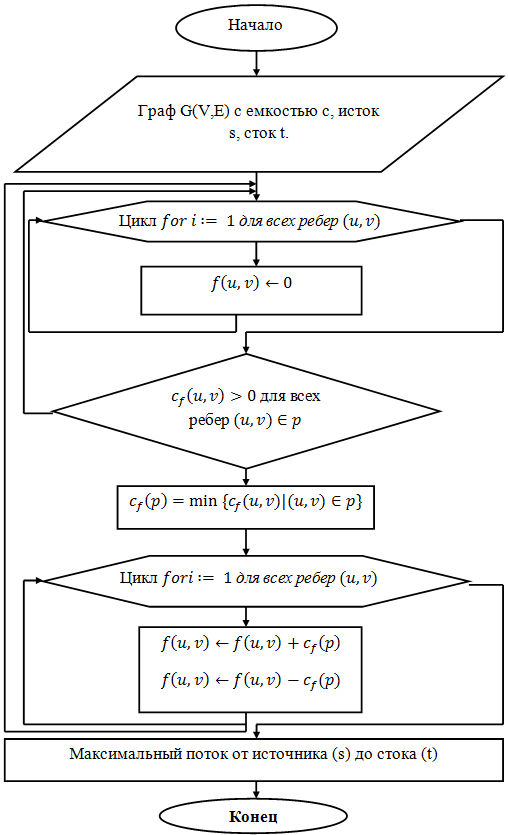
\includegraphics [scale=1] {images/h12.png}
\begin{center}
%\captionsetup{justification=justified, labelsep=period}
\caption{Блок-схема алгоритма разреза на графах.} \label{img12}
\end{center}
\end{figure}

Метод разреза графов находит сильные локальные минимумы энергетической функции. Метод достаточно мощный, чтобы решать множество полезных задач, и он может быть применен к решению проблемы графика min-среза. 
\begin{equation}\label{eq25}
E\left(f\right) = \sum_{p \in P}D_p\left(f_p\right)+\sum_{p,q \in N}V_{p,q}\left(f_p,f_q\right).
\end{equation}
Найти маркировки $f:P\rightarrow L$ , что сводит к минимуму $E\left(f\right)$ из множеств пикселей $P$, набор этикеток $L,N \in P$ является система соседства по пикселям. $D_p\left(f_p\right)$ является функцией, которая получена из данных наблюдений, и которая измеряет стоимость присвоения метки $f_p$ на пиксель $p$. $V_{\left(p,q\right)} \left(f_p,f_q\right)$ , и измеряет стоимость присвоения метки $f_p$,$f_q$ на соседние пиксели $p$, $q$. Используется для улучшения пространственного сглаживания \cite{Boykovv2001, Boykov2004}.

На каждом шаге алгоритм выполняет каждый поток, который соединяет от $s$ к $t$. Сложность алгоритма зависит от числа ребер, осуществляется по индукции всех потоков. Движение потока увеличивается, по меньшей мере один раз на каждом шаге алгоритма. Поэтому, сложность алгоритма не превосходит $O\left(f\right)$, где  $f$ - максимальный поток в графе.  $E$ - это число ребер графа, так что сложность будет $О\left(E\ast f\right)$.

После этого в полученном графе находится минимальный разрез, который делит граф на $2$ части. Вес ребер между метками обеспечивает выполнение заданных пользователем ограничений: маркировки объекта будут отнесены к объекту, маркировки фона - к фону.

%-------------------------
\subsection{Итеративный алгоритм ближайших точек}
Итеративный алгоритм ближайших точек Paul J. Besl и Neil D. Mackay представили в научном журнале IEEE впервые в феврале 1992 года \cite{Besl1992}. Итеративный алгоритм ближайших точек  используется для минимизации расстояния между двумя заданными точками. Алгоритм широко используется в построения на основе изображения 3D \cite{Gelfan2003, Rusinkiewicz2001}. Для сокращения времени вычислений и улучшить сходимость итерационных ближайшей точки (ICP) в ключевых точках экстракции. В каждой итерации $ICP$, то RANSAC \cite{Hast2013} вкладывается, чтобы удалить выбросы и сходимость $ICP$ гарантируется.  Алгоритм $RANSAC$ часто используется в компьютерном зрении. Преимуществом алгоритма $RANSAC$ является его способность дать надёжную оценку параметров модели, то есть возможность оценить параметры модели с высокой точностью, даже если в исходном наборе данных присутствует значительное количество выбросов.
В данной работе алгоритм $ICP$ используется чтобы уменьшить отклонение конкретных точек на контуре человеческой части. Созданный набор признаков используется для сравнения с множеством точек, извлечённых с объекта. Для простого сравнения потребуется время и ресурсы системы. Результаты получаются не такие, как ожидались. Форма движения и шум будут влиять на результаты работы программы. Таким образом, чтобы преодолеть эту проблему используется алгоритм $ICP$, чтобы уменьшить различия между этими двумя наборами точек.

Полученным результатом является набор признаков объекта, находящегося близко к контуру 2D тела человека на фотографии. Мы провели уточнения контура пикселей на объекте с помощью алгоритма $ICP$ (рис \ref{img13}).
\begin{figure}[ht!]
\centering
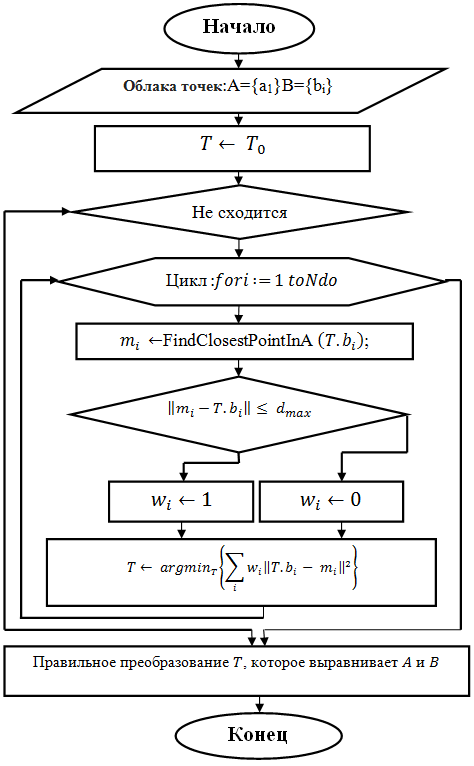
\includegraphics [scale=1] {images/h13.png}
\begin{center}
%\captionsetup{justification=justified, labelsep=period}
\caption{Блок-схема алгоритма $ICP$} \label{img13}
\end{center}
\end{figure}
В набор точек признаков, найденных на объекте, $29$ точек имеют признаки, извлеченные с атрибутами характерной геометрии: выпуклые, вогнутые кривые, соответствующие важным позициям, связанными с измерением размеров частей тела. Алгоритм включает в себя основные шаги:

\begin{itemize}
	\item \textbf{Шаг 1:} Вычислим соответствия между двумя сканированиями;
	\item \textbf{Шаг 2:} Выполним преобразование, которое сводит к минимуму расстояние между соответствующими точками.
\end{itemize}
Используем соответствующее максимальное пороговое значение $d_{max}$. Здесь $d_{max}$ представляет собой баланс между сходимостью и точностью.

Алгоритм $ICP$ повторяет действия, чтобы минимизировать среднеквадратичную ошибку пикселов, соответствующих ближайшей точке.
\begin{equation}\label{eq26}
T\leftarrow argmin_t\left\{\sum_i\left\|T.b_i - m_i\right\|^2\right\}.
\end{equation}
Где:

\begin{itemize}
	\item $T$ - правильное преобразование;
	\item $b_i$: $B=\left\{b_i\right\}$ - Облака точек;
	\item $m_i$ - множество точек, которые будут преобразованы из $B$ - $A$ ( $A=\left\{a_i\right\}$ - Облака точек);
\end{itemize}

Набор новых точек будет найден, если он удовлетворяет двум условиям:

\begin{itemize}
	\item Расположен на границе или наиболее близко к границам объекта;
	\item Расстояние между двумя наборами точек является наименьшим.
\end{itemize}
Таким образом, получен набор новых признаков для описания точного контура объекта.

Этапы алгоритма ICP выполнются последовательно. Алгоритм остановится только, если имеет место сходимость (наименьшая ошибка и стабильность). Алгоритм $ICP$ с такими операциями всегда монотонно сходится на интервале области определения функции. Тем не менее параметры алгоритма зависят от настройки. Таким образом, алгоритм $ICP$ будет сходиться на всей области определения функции. В то же время, новые точки признаков абсолютно совпадают с точками признаков в базе данных.
%-------------------------
\subsection{Извлечение антропометрических признаков из видео}
Для решения задачи извлечения антропометрических признаков с изображения и видео предложен алгоритм, основанный на  комбинации новейших методов - технике предварительной обработки изображений, алгоритме вычитания фона, алгоритме сегментации изображений на основе разреза графов, алгоритме итеративных ближайших точек.

Процесс извлечения антропометрических признаков объектов на изображении и видео на основе алгоритма компьютерного зрения включает в себя следующие этапы (рис \ref{img14}):
\begin{itemize}
	\item \textbf{Шаг 1:} Предварительная обработка изображения;
	
	\begin{itemize}
		\item Фильтр шума с гауссовым фильтром с матрицей фильтра окна $\left[5 5\right]$;
		\item Используем морфологические операторы - дилатации, чтобы улучшить качество точек изображения со структурами элементов $se=strel\left(line,11,90\right)$;
		\item Эквализация гистограммы.
	\end{itemize}
	\item \textbf{Шаг 2:} Обнаружение объекта и человеческого лица. Важную роль на этом шаге играет алгоритм вычитания фона. Расчетные значения пикселей на разных кадрах получаем по формуле (\ref{eq9});
	
	Метод Виола-Джонса \cite{Violaj2001, Viola2004} используется для обнаружения человеческого лица с изображения. Метод состоит из трех основных этапов: интегральном представлении изображения, метод построения классификатора на основе алгоритма адаптивного бустинга (AdaBoost) и метод комбинирования классификаторов в каскадную структуру.
	\item \textbf{Шаг 3:} Сегментация изображения методом разреза на графах. Поиск области изображения, содержащего части тела человека на основе формулы (\ref{eq25});
	\item \textbf{Шаг 4:} Обнаружение контура и поиск ключевых точек признаков – алгоритм $ICP$. Расчет евклидова расстояния: $d\left(A,B\right) = \sqrt{\left(x_B - x_A\right)^2 + \left(y_B - y_A\right)^2}$;
	\item \textbf{Шаг 5:} Создание антропометрического вектора признаков.
\end{itemize}

\begin{figure}[ht!]
\centering
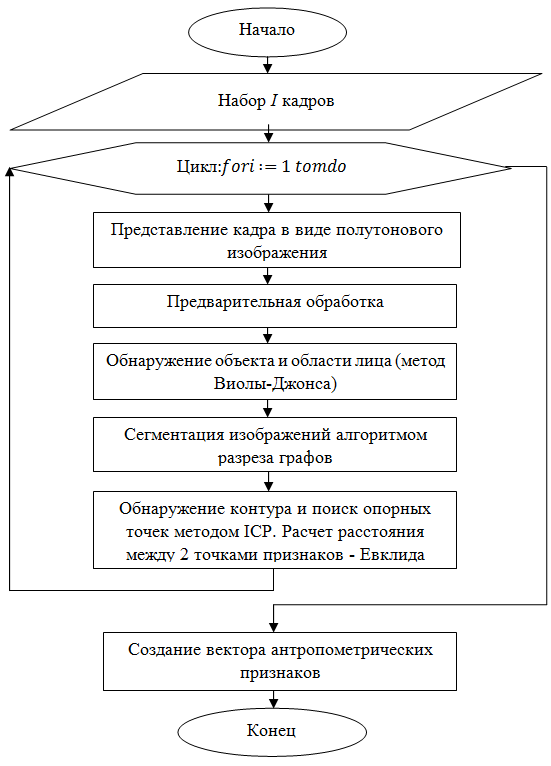
\includegraphics [scale=1.05] {images/h14.png}
\begin{center}
%\captionsetup{justification=justified, labelsep=period}
\caption{Блок-схема алгоритма извлечения антропометрических признаков из видеопоследовательности.} \label{img14}
\end{center}
\end{figure}
%-------------------------